\documentclass[aspectratio=169,11pt,t]{beamer}
% ============================================================
%  ksa-cs-v2: ksa-cs-lecture-template.tex 스타일 + 한글, v2 덱(16:9)용.
%    - 짙은 네이비 헤드라인 (섹션 이름 + 프레임마다 점)
%    - 꽉 찬 파란 제목 막대, 둥근 그림자 블록
%    - 한글: Noto Sans CJK KR (fontspec)
%  사용:
%    \documentclass[aspectratio=169,11pt,t]{beamer}
%    \input{<..>/theme/ksa-cs-v2.tex}
%  ksa-theme.tex 의 매크로(\kb \kq, ksablue/ksared 등)도 같은 이름으로 둔다
%  -> v2 덱 본문을 거의 그대로 옮길 수 있다.
% ============================================================

\usepackage{fontspec}
\usepackage{amsmath,amssymb}
\usepackage{tikz}
\usepackage{listings}
\usepackage{graphicx}
\usepackage{booktabs}
\usepackage{varwidth}
% enumitem 은 넣지 않는다 (beamer 글머리표가 사라진다)

\defaultfontfeatures{Ligatures=TeX}
\setmainfont{Noto Sans CJK KR}
\setsansfont{Noto Sans CJK KR}
\setmonofont{Noto Sans Mono CJK KR}[Scale=0.92]
\usefonttheme{professionalfonts}

% ---------- 기본 틀 ----------
\usetheme{default}
\useinnertheme[shadow=true]{rounded}
\setbeamertemplate{navigation symbols}{}
\setbeamersize{text margin left=1em,text margin right=1em}

% ---------- 색 (템플릿 원본 값) ----------
\definecolor{navydark}{HTML}{191959}
\definecolor{navydim}{HTML}{8888B0}
\definecolor{navytitle}{HTML}{262686}
\definecolor{navyblue}{HTML}{3333B2}
\definecolor{blockbodybg}{HTML}{E9E9F3}
\definecolor{examplegreen}{HTML}{006000}
\definecolor{examplebg}{HTML}{E5EFE5}
\definecolor{alertred}{HTML}{BF0000}
\definecolor{alertbg}{HTML}{F9E5E5}
% ksa-theme.tex 와 같은 이름 (본문 호환)
\colorlet{ksablue}{navytitle}
\colorlet{ksabluedk}{navydark}
\definecolor{ksagold}{HTML}{D6CBB1}
\definecolor{ksagolddk}{HTML}{A9976B}
\colorlet{ksared}{alertred}
\definecolor{ksagray}{HTML}{5B5B5B}

\setbeamercolor{structure}{fg=navyblue}
\setbeamercolor{alerted text}{fg=alertred}
\setbeamercolor{frametitle}{bg=navytitle,fg=white}
\setbeamercolor{title}{fg=white,bg=navytitle}
\setbeamercolor{block title}{bg=navytitle,fg=white}
\setbeamercolor{block body}{bg=blockbodybg,fg=black}
\setbeamercolor{block title example}{bg=examplegreen,fg=white}
\setbeamercolor{block body example}{bg=examplebg,fg=black}
\setbeamercolor{block title alerted}{bg=alertred,fg=white}
\setbeamercolor{block body alerted}{bg=alertbg,fg=black}
\setbeamercolor{item}{fg=navyblue}
\setbeamertemplate{itemize item}[circle]
\setbeamertemplate{itemize subitem}[triangle]

% ---------- 헤드라인: miniframes (섹션 이름 + 점) ----------
\useoutertheme[subsection=false]{miniframes}
\setbeamerfont{section in head/foot}{size=\tiny}
\setbeamercolor{section in head/foot}{bg=navydark,fg=white}
\setbeamercolor{mini frame}{fg=white}
\setbeamertemplate{mini frames}[circle]

% ---------- 제목 막대: 폭 꽉 채움, 두 줄까지 ----------
\setbeamerfont{frametitle}{size=\normalsize,series=\bfseries}
\setbeamertemplate{frametitle}{%
  \nointerlineskip
  \begin{beamercolorbox}[wd=\paperwidth,ht=2.7ex,dp=1.1ex,leftskip=.3cm,rightskip=.3cm]{frametitle}%
    \usebeamerfont{frametitle}\insertframetitle
  \end{beamercolorbox}}

% ---------- 쪽 번호: 오른쪽 아래 ----------
\setbeamertemplate{footline}{%
  \hfill
  {\color{navydim}\scriptsize\insertframenumber\,/\,\inserttotalframenumber}%
  \hspace{3mm}\vspace{2mm}%
}

% ---------- 표지: 템플릿처럼 헤드라인은 그대로, 가운데 둥근 그림자 상자에 제목 한 줄 ----------
% 덱에서:  {\setbeamertemplate{footline}{}\begin{frame}[c,noframenumbering]\titlepage\end{frame}}
\setbeamercolor{title}{fg=white,bg=navyblue}
\makeatletter
\setbeamertemplate{title page}{%
  \vfill
  \centering
  \begin{minipage}{0.84\paperwidth}
  \begin{beamercolorbox}[wd=\linewidth,sep=7pt,center,rounded=true,shadow=true]{title}
    {\usebeamerfont{title}\inserttitle\par}%
    \ifx\insertsubtitle\@empty\else\vskip0.4em{\usebeamerfont{subtitle}\insertsubtitle\par}\fi
  \end{beamercolorbox}
  \end{minipage}\par\vskip1.6em
  {\usebeamerfont{author}\color{navytitle}\insertauthor\par}\vskip0.3em
  {\usebeamerfont{institute}\color{ksagray}\insertinstitute\par}
  \vfill
}
\makeatother
\setbeamerfont{title}{series=\bfseries,size=\Large}
\setbeamerfont{subtitle}{size=\normalsize}
\setbeamerfont{author}{size=\normalsize}
\setbeamerfont{institute}{size=\small}

% ksa-theme 호환: 덱이 \renewcommand{\ksacredit}{..} 를 해도 되게 (꼬리말에는 안 쓴다)
\newcommand{\ksacredit}{}

% ---------- 강조 ----------
\newcommand{\hl}[1]{\textcolor{alertred}{#1}}
\newcommand{\hlb}[1]{\textcolor{navyblue}{#1}}
\newcommand{\kb}[1]{\textbf{\color{ksablue}#1}}
\newcommand{\kq}[1]{\textbf{\color{ksared}#1}}

% ---------- 파이썬 코드 (템플릿과 같은 색) ----------
\definecolor{codekw}{HTML}{0033B3}
\definecolor{codebuiltin}{HTML}{BF0000}
\definecolor{codestr}{HTML}{067D17}
\definecolor{codecomment}{HTML}{8C8C8C}
\definecolor{codenum}{HTML}{1750EB}
\lstdefinestyle{py}{
  language=Python, basicstyle=\ttfamily\scriptsize,
  keywordstyle=\color{codekw}\bfseries, stringstyle=\color{codestr},
  commentstyle=\color{codecomment}\itshape, numberstyle=\color{codenum},
  emph={print,len,range,sum,input,int,str,float,list,dict,append,remove,sorted,abs,min,max},
  emphstyle=\color{codebuiltin}, showstringspaces=false, keepspaces=true,
  columns=fixed, basewidth=0.52em, aboveskip=1mm, belowskip=1mm, xleftmargin=2mm,
  breaklines=true
}
\lstset{style=py}

% 원본 덱 (ksa-theme): slides/v2/ml1/week15/diffusion/ -- 그림은 거기 figs/ 를 그대로 쓴다
\setbeamerfont{author}{size=\normalsize}
\setbeamerfont{institute}{size=\small}
\graphicspath{{../../../v2/ml1/week15/diffusion/figs/}{../../../assets/}}
\makeatletter
\newcommand{\markpage}[1]{\protected@write\@auxout{}{\string\newlabel{#1}{{\the\c@framenumber}{}}}\hypertarget{#1}{}}
\newcommand{\pref}[1]{\hyperlink{#1}{\textcolor{ksagolddk}{(p.\ref{#1})}}}
\makeatother

\renewcommand{\ksacredit}{Machine Learning and Deep Learning \,\textperiodcentered\, 확산 모델}
\title{Diffusion 확산 모델}
\subtitle{노이즈를 조금씩 지워 그림을 만든다}
\author{Machine Learning and Deep Learning}
\institute{한국과학영재학교 (KSA)}
\date{}
\begin{document}
{\setbeamertemplate{footline}{}\begin{frame}[c,noframenumbering]\titlepage\end{frame}}


\section{질문}
% --- 오늘의 질문
\begin{frame}{오늘의 질문: 노이즈에서 고양이가 나올 수 있을까?}
\vfill
\centering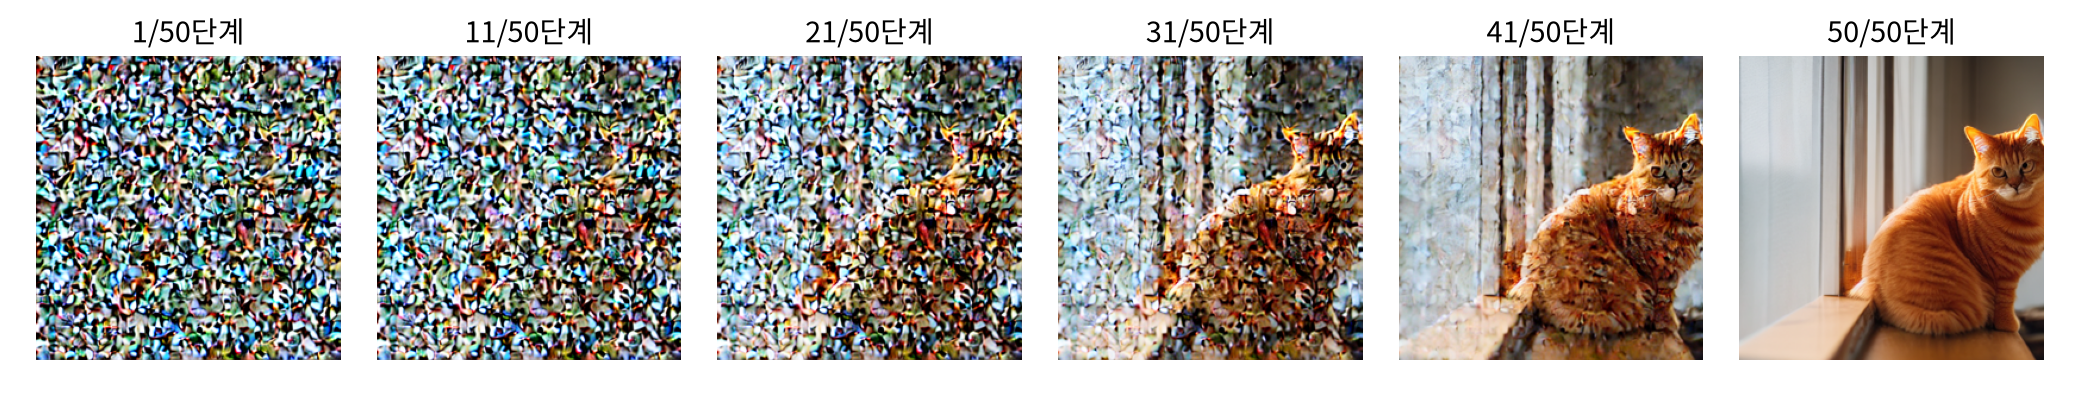
\includegraphics[width=0.94\linewidth]{df_reverse.png}\par\vskip0.3em
{\normalsize ``a photo of an orange tabby cat sitting on a wooden windowsill'' (Stable Diffusion v1.5)}\\[0.4em]
{\large 잉크가 물에 \textbf{퍼지듯 (diffusion)} 노이즈를 퍼뜨린 것을 거꾸로}
\vfill
\note{무작위 노이즈에서 시작해 50단계에 걸쳐 조금씩 지웠더니 창가에 앉은 주황 고양이가 나타났습니다. 오픈소스 Stable Diffusion을 직접 돌린 결과입니다. 확산 모델이라는 이름은 잉크가 물에 퍼지듯 그림에 노이즈를 퍼뜨리는 과정에서 왔습니다. 이 모델은 그 반대, 퍼진 노이즈를 거둬들이는 법을 배웁니다. 지금 그림 생성 AI 대부분이 이 방법입니다.}
\end{frame}

\section{섞기}
% --- 앞으로
\begin{frame}{앞으로: 노이즈를 1,000번 나눠 섞는다}
\markpage{forward}
\vfill
\centering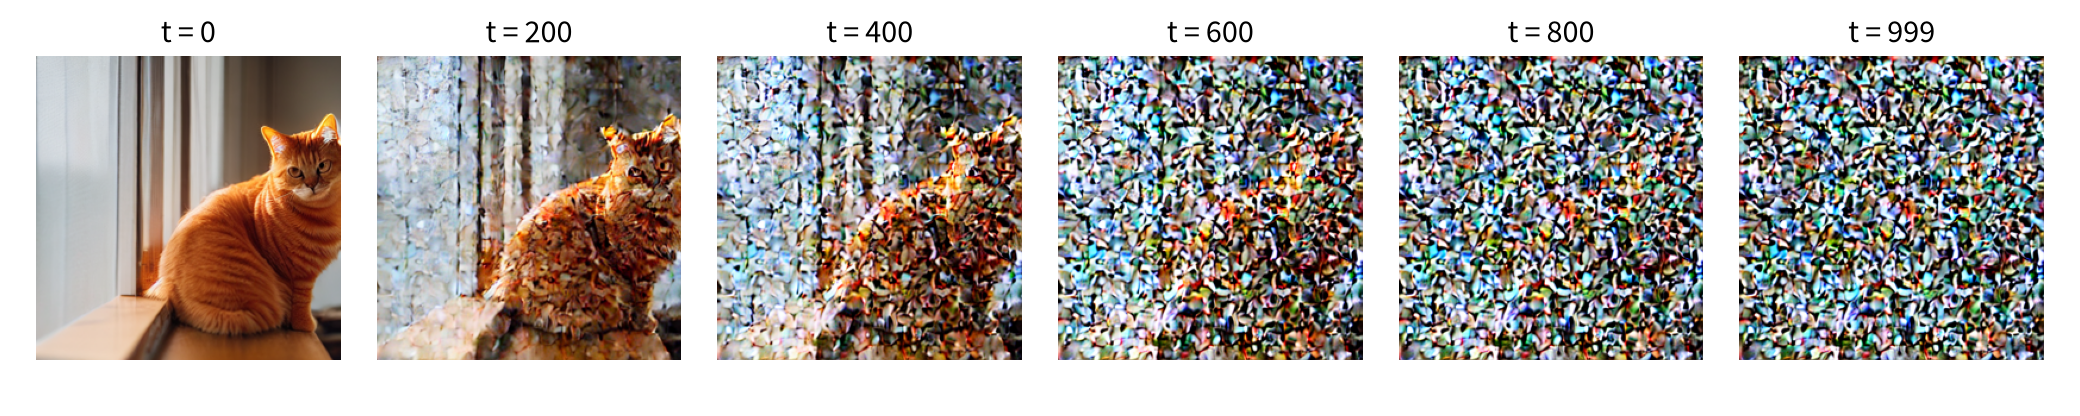
\includegraphics[width=0.94\linewidth]{df_forward.png}\par\vskip0.2em
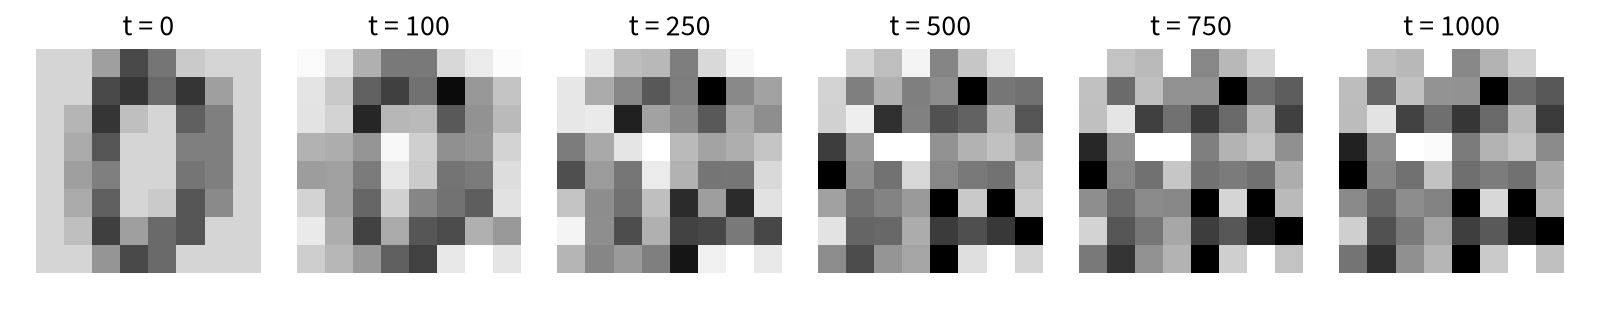
\includegraphics[width=0.66\linewidth]{df_digit_fwd.png}\par
{\large 한 번에 아주 조금씩 ($\beta$: 0.0001 $\to$ 0.02) \quad $t = 1000$ 이면 원래 그림은 거의 남지 않는다}
\vfill
\note{먼저 앞으로 가는 과정입니다. 완성된 그림에 노이즈를 1000번에 나눠 조금씩 섞습니다. 한 번에 섞는 양 베타는 0.0001에서 0.02로 천천히 늘어납니다. 고양이 사진도, 아래 손글씨 0도 t가 커질수록 흐려져 1000번째에는 원래 그림이 거의 남지 않고 순수한 노이즈가 됩니다. 이 과정에는 학습할 것이 없습니다. 그냥 섞기만 하면 됩니다.}
\end{frame}

% --- 식
\begin{frame}{식으로: 한 번에 $t$ 단계까지 섞기}
\markpage{formula}
\vfill
\begin{columns}[c]
\column{0.5\linewidth}\centering
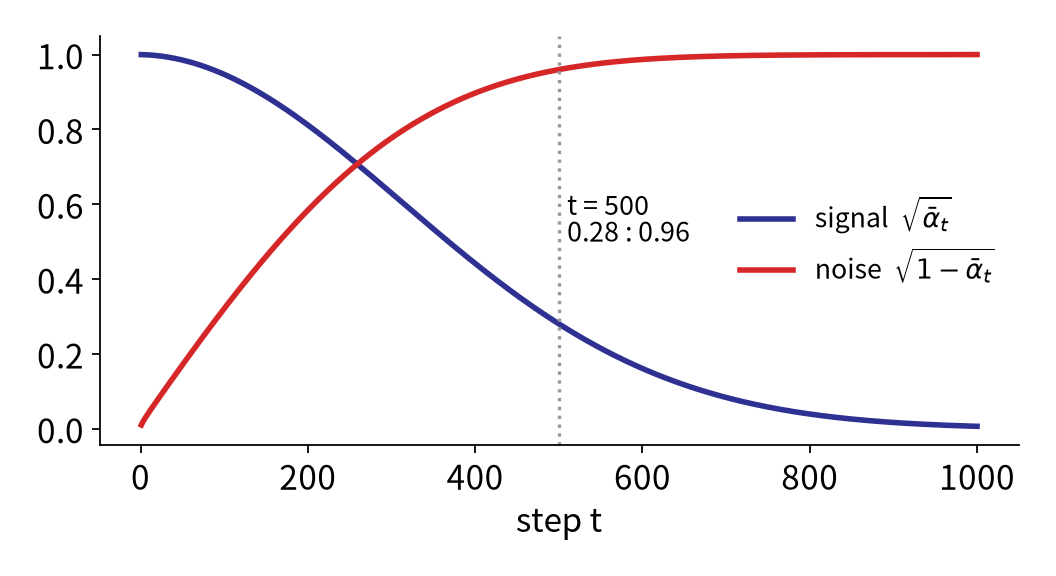
\includegraphics[width=\linewidth]{df_schedule.png}
\column{0.48\linewidth}
{\Large\[ \mathbf{x}_t = \sqrt{\bar\alpha_t}\, \mathbf{x}_0 + \sqrt{1 - \bar\alpha_t}\; \boldsymbol{\epsilon} \]}
{\large $\boldsymbol{\epsilon} \sim N(0, 1)$ \quad $\bar\alpha_t = \prod_{s \le t} (1 - \beta_s)$}\\[0.6em]
{\large 손 계산: $t = 500$ 이면 $\bar\alpha = 0.079$}\\
{\large 그림 $\times$ \kb{0.28} $+$ 노이즈 $\times$ \kq{0.96}}\\[0.4em]
{\small 1,000번을 일일이 안 해도 바로 $t$ 단계 그림을 만든다}
\end{columns}
\vfill
\note{식으로 보면, t단계까지 섞은 그림은 원래 그림에 루트 알파바를, 노이즈에 루트 1 빼기 알파바를 곱해 더한 것입니다. 알파바는 1 빼기 베타를 t번 곱한 값입니다. 그래서 1000번을 일일이 섞지 않아도 원하는 단계의 그림을 한 번에 만들 수 있습니다. t가 500이면 알파바가 0.079라, 원래 그림이 0.28배, 노이즈가 0.96배 들어 있습니다. 반쯤 왔는데 벌써 노이즈가 훨씬 많습니다.}
\end{frame}

% --- 학습
\begin{frame}{학습: 섞인 노이즈를 맞힌다}
\markpage{train}
\vfill
\centering
\renewcommand{\arraystretch}{1.5}
{\large\begin{tabular}{rl}
1 & 데이터에서 그림 $\mathbf{x}_0$, 단계 $t$ (1 $\sim$ 1,000), 노이즈 $\boldsymbol{\epsilon}$ 를 뽑는다\\
2 & 섞는다: $\mathbf{x}_t = \sqrt{\bar\alpha_t}\, \mathbf{x}_0 + \sqrt{1 - \bar\alpha_t}\, \boldsymbol{\epsilon}$\\
3 & 신경망이 $(\mathbf{x}_t, t)$ 를 보고 노이즈를 맞힌다: $\hat{\boldsymbol{\epsilon}} = f(\mathbf{x}_t, t)$\\
4 & 손실 $= \|\hat{\boldsymbol{\epsilon}} - \boldsymbol{\epsilon}\|^2$ \quad (평균 제곱 오차, 1주차부터 본 그것)
\end{tabular}}\vskip0.6em
{\large GAN 처럼 겨루지 않는다: 손실이 하나라 \kb{안정적}으로 학습된다}\\[0.2em]
{\small Ho, Jain, Abbeel (2020) DDPM \quad 처음 제안: Sohl-Dickstein 외 (2015)}
\vfill
\note{학습은 놀랄 만큼 단순합니다. 데이터에서 그림 하나, 단계 t 하나, 노이즈 하나를 뽑아 섞고, 신경망이 섞인 그림과 t를 보고 어떤 노이즈가 섞였는지 맞히게 합니다. 손실은 맞힌 노이즈와 진짜 노이즈의 평균 제곱 오차입니다. 1주차부터 봐 온 그 손실이죠. GAN처럼 두 신경망이 겨루지 않으니 학습이 안정적입니다. 2015년 솔딕스타인 팀이 처음 제안했고, 2020년 호, 자인, 아빌의 DDPM 논문이 이 단순한 손실로 품질을 크게 끌어올렸습니다.}
\end{frame}

\section{되돌리기}
% --- 뒤로
\begin{frame}{뒤로: 노이즈에서 시작해 조금씩 지운다}
\vfill
\centering
{\Large\[ \mathbf{x}_{t-1} = \frac{1}{\sqrt{1 - \beta_t}} \Big( \mathbf{x}_t - \frac{\beta_t}{\sqrt{1 - \bar\alpha_t}}\, f(\mathbf{x}_t, t) \Big) + \sqrt{\beta_t}\, \mathbf{z} \]}\vskip0.4em
\renewcommand{\arraystretch}{1.4}
{\large\begin{tabular}{rl}
1 & 순수한 노이즈 $\mathbf{x}_{1000}$ 에서 시작\\
2 & 신경망이 맞힌 노이즈를 \textbf{조금} 뺀다 (그리고 새 노이즈를 아주 조금 더한다)\\
3 & $t = 1000, 999, \dots, 1$ 까지 되풀이 $\to$ 그림
\end{tabular}}\vskip0.4em
{\large 단계마다 시작 노이즈가 다르면 \textbf{다른 그림}: 무한히 다양하게}
\vfill
\note{그림을 만들 때는 거꾸로 갑니다. 순수한 노이즈에서 시작해, 신경망이 이 단계에 섞여 있다고 맞힌 노이즈를 조금 빼고, 새 노이즈를 아주 조금 더합니다. 이걸 1000단계부터 1단계까지 되풀이하면 그림이 나타납니다. 시작 노이즈가 다르면 다른 그림이 나오니 끝없이 다양한 그림을 만들 수 있습니다. 대신 신경망을 1000번 돌려야 하니 느립니다.}
\end{frame}

% --- 실험
\begin{frame}{실험: 손글씨 숫자 확산 모델}
\markpage{exp}
\vfill
\centering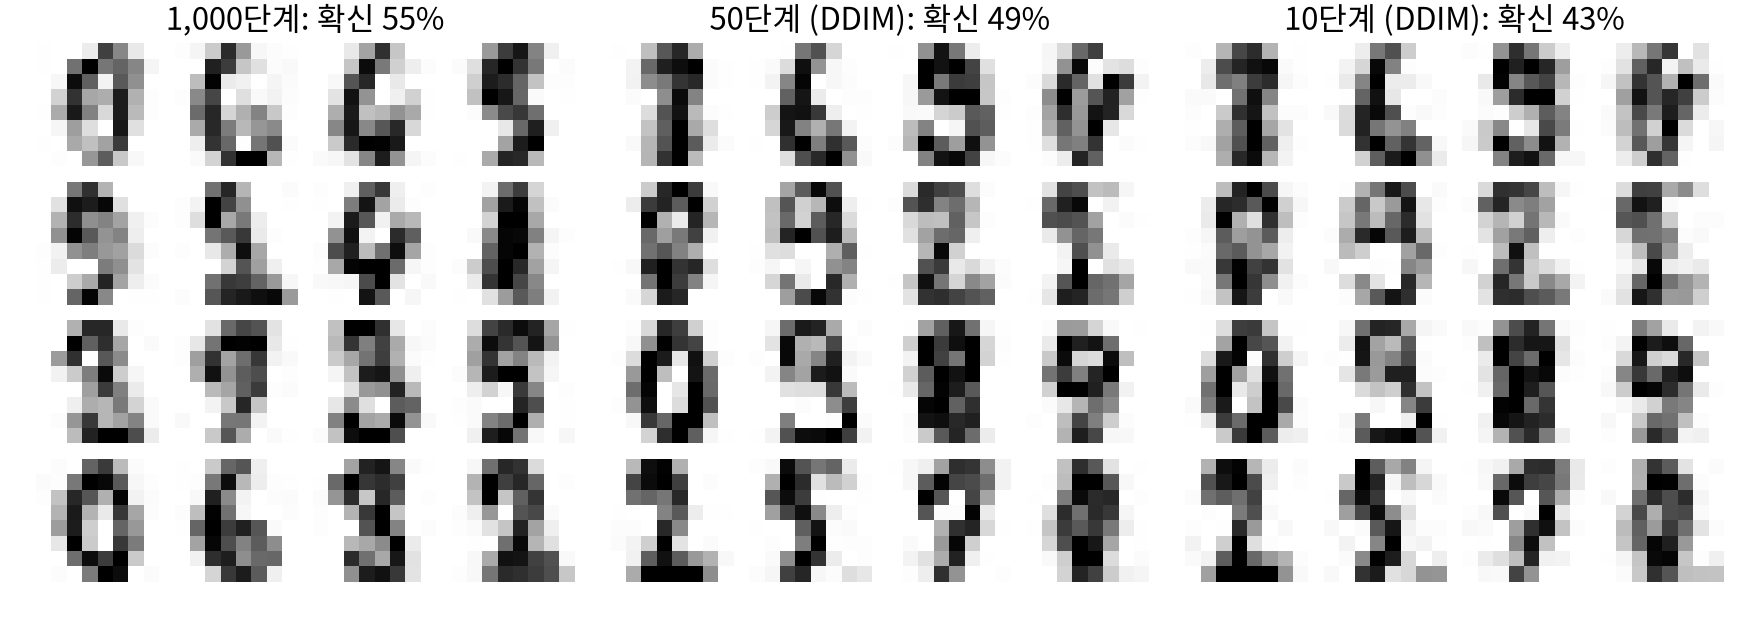
\includegraphics[width=0.8\linewidth]{df_digits.png}\par\vskip0.1em
\renewcommand{\arraystretch}{1.25}
{\large\begin{tabular}{lccccc}
같은 판정으로 & VAE & GAN & \textbf{확산} (1,000단계) & 50단계 & 원본 사진\\\hline
분류기 확신 (0.9 이상) & 31\% & 36\% & \kb{55\%} & 49\% & 77\%\\
숫자 종류 & 10 & 10 & 10 (175 $\sim$ 225장씩) & 10 &
\end{tabular}}
\vfill
\note{손글씨 숫자로 작은 확산 모델을 직접 학습했습니다. 노트북 CPU로 약 70초입니다. 2000장을 만들어, VAE와 GAN 덱과 같은 분류기로 판정했습니다. 분류기가 0.9 이상 확신한 비율은 VAE 31퍼센트, GAN 36퍼센트, 확산 모델 55퍼센트로, 원본 사진 77퍼센트에 가장 가깝습니다. 열 종류 숫자도 175장에서 225장씩 고르게 나왔습니다. 모드 붕괴가 없습니다.}
\end{frame}

\section{빠르게}
% --- 빠르게
\begin{frame}{1,000번은 너무 많다: 건너뛰기}
\vfill
\centering
\renewcommand{\arraystretch}{1.4}
{\large\begin{tabular}{lccc}
뽑는 방법 & 신경망 실행 & 2,000장 시간 (CPU) & 확신\\\hline
DDPM & 1,000번 & 3.9초 & 55\%\\
DDIM (Song 외 2020) & \kb{50}번 & \kb{0.16}초 & 49\%\\
DDIM & 10번 & 0.03초 & 43\%
\end{tabular}}\vskip0.8em
{\large 같은 신경망을 다시 학습하지 않고, 단계를 건너뛰며 지운다}\\[0.2em]
{\large Stable Diffusion 기본값도 50단계 \quad 1 $\sim$ 4단계로 줄이는 연구도}
\vfill
\note{1000번 신경망을 돌리는 건 느립니다. 2020년 DDIM은 같은 신경망을 그대로 쓰면서 단계를 건너뛰며 지우는 방법을 냈습니다. 우리 숫자 모델로 재 보니 1000단계는 2000장에 3.9초, 50단계는 0.16초로 약 25배 빠르고 확신은 55에서 49퍼센트로 조금 낮아졌습니다. 10단계는 43퍼센트입니다. Stable Diffusion의 기본값도 50단계이고, 요즘은 1에서 4단계까지 줄이는 연구도 많습니다.}
\end{frame}

% --- Stable Diffusion
\begin{frame}{Stable Diffusion: 압축된 공간에서, 글을 따라}
\vfill
\centering
\renewcommand{\arraystretch}{1.6}
{\large\begin{tabular}{ll}
압축 (2021) & 512 × 512 × 3 $\to$ 64 × 64 × 4 (\kb{48분의 1}) 에서 확산\\
& 오토인코더로 줄였다가 마지막에 되살린다 (VAE 덱)\\
글 조건 & CLIP 글 임베딩 (임베딩 덱) 을 어텐션 (12주차) 으로 넣는다\\
guidance 7.5 & 글 있을 때 · 없을 때 예측 차이를 7.5배로
\end{tabular}}\vskip0.6em
{\large 이번 학기에 배운 조각들이 한 모델에 모였다}
\vfill
\note{Stable Diffusion은 세 가지를 더했습니다. 첫째, 512 곱하기 512 그림을 오토인코더로 64 곱하기 64 곱하기 4, 48분의 1로 줄인 공간에서 확산을 해 훨씬 빠릅니다. 2021년 롬바흐 팀의 잠재 확산입니다. 둘째, 글을 CLIP의 글 임베딩으로 바꿔 어텐션으로 신경망에 넣어, 글을 따르는 그림을 만듭니다. 셋째, guidance 7.5는 글이 있을 때와 없을 때의 예측 차이를 7.5배 키워 글을 더 잘 따르게 합니다. VAE, 임베딩, 어텐션, 이번 학기에 배운 조각들이 한 모델에 모였습니다.}
\end{frame}

% --- 역사
\begin{frame}{확산 모델의 길}
\vfill
\centering
\renewcommand{\arraystretch}{1.5}
{\large\begin{tabular}{ll}
2015 & Sohl-Dickstein 외: 물리학 (비평형 열역학) 에서 온 생각\\
2020 & DDPM: 노이즈 맞히기로 GAN 수준의 그림 \quad DDIM: 빠르게\\
2021 $\sim$ 2022 & 잠재 확산 · Stable Diffusion (공개), DALL·E 2, Imagen\\
2024 $\sim$ & 동영상 (Sora 등), 단백질 구조 설계 (RFdiffusion), 음악
\end{tabular}}\vskip0.8em
{\large 장점: 안정적 학습, 다양하고 선명 \quad 약점: 여러 번 돌려야 해서 느리다}
\vfill
\note{확산 모델은 2015년 물리학의 비평형 열역학에서 온 생각으로 처음 제안됐고, 2020년 DDPM이 노이즈 맞히기로 GAN 수준의 그림을 만들었습니다. 2021년과 2022년에는 잠재 확산과 Stable Diffusion이 공개되고, DALL-E 2와 Imagen이 나왔습니다. 지금은 동영상, 단백질 구조 설계, 음악까지 확산 모델로 만듭니다. 장점은 안정적인 학습과 다양하고 선명한 결과, 약점은 신경망을 여러 번 돌려야 해서 느리다는 점입니다.}
\end{frame}

\section{연습}
% --- 문제풀이
\begin{frame}{문제풀이}
\vfill
\begin{enumerate}
\item $\bar\alpha_t = 0.36$ 이면 $\mathbf{x}_t$ 에 그림과 노이즈가 각각 몇 배 들어 있나?\vskip0.8em
\item $\mathbf{x}_0 = 1$, $\epsilon = -1$, $\bar\alpha_t = 0.64$ 이면 $x_t$ 는?\vskip0.8em
\item 학습할 때 $t$ 를 1,000 하나로만 뽑으면 어떤 문제가 생길까?\vskip0.8em
\item 확산 모델이 GAN 보다 모드 붕괴가 적은 이유를 학습 방법으로 설명해 보라.
\end{enumerate}
\vfill
\note{1번 답. 그림은 루트 0.36, 0.6배, 노이즈는 루트 0.64, 0.8배입니다. 2번 답. 0.8 곱하기 1 더하기 0.6 곱하기 마이너스 1, 0.2입니다. 3번 답. 거의 순수한 노이즈만 보니 그림의 모양을 배울 수 없고, 거꾸로 지울 때 중간 단계를 처리하지 못합니다. 4번 답. 모든 데이터 그림에 노이즈를 섞어 맞히는 손실 하나를 줄이니, 데이터의 모든 종류를 고르게 배웁니다. 판별자의 약한 곳만 노리는 경쟁이 없습니다.}
\end{frame}

% --- 실습
\begin{frame}{실습}
\vfill
\centering\begin{tabular}{rl}
\large 1 & 노이즈 스케줄: $\bar\alpha_t$, 한 번에 $t$ 단계까지 섞기\\[0.5em]
\large 2 & 손글씨 숫자 DDPM 학습 (노이즈 맞히기)\\[0.5em]
\large 3 & 1,000단계 vs 50단계로 그림 만들기, 종류 · 확신 세기
\end{tabular}\vskip1em
\href{https://colab.research.google.com/github/SuminHan/book-ml/blob/main/slides/v2/ml1/week15/diffusion/lab/diffusion.ipynb}{\textcolor{ksagolddk}{▶ Colab에서 실습 노트북 열기}}
\vfill
\note{실습은 세 부분입니다. 첫째, 노이즈 스케줄을 만들고 한 번에 t단계까지 섞어 봅니다. 둘째, 손글씨 숫자로 작은 DDPM을 학습합니다. 셋째, 1000단계와 50단계로 그림을 만들고 종류와 확신을 셉니다.}
\end{frame}

\section{정리}
% --- 정리
\begin{frame}{정리}
\vfill
\centering\large\begin{tabular}{l}
\textbf{확산 모델}: 노이즈를 1,000번 나눠 섞고, 섞인 노이즈를 맞히도록 학습\\[0.5em]
$\mathbf{x}_t = \sqrt{\bar\alpha_t}\mathbf{x}_0 + \sqrt{1-\bar\alpha_t}\boldsymbol\epsilon$ \quad 손실 = 노이즈의 평균 제곱 오차\\[0.5em]
숫자: 확신 VAE 31\% · GAN 36\% · 확산 \kb{55\%} \quad DDIM 50단계 약 25배 빠르게\\[0.5em]
Stable Diffusion = 48분의 1 압축 + CLIP 글 + 어텐션
\end{tabular}
\vfill
\note{정리합니다. 확산 모델은 그림에 노이즈를 1000번 나눠 섞고, 섞인 노이즈를 맞히도록 학습한 뒤, 노이즈에서 시작해 조금씩 지워 그림을 만듭니다. 손실은 노이즈의 평균 제곱 오차 하나라 안정적입니다. 숫자 실험에서 같은 판정으로 VAE 31, GAN 36, 확산 55퍼센트였고 열 종류가 고르게 나왔으며, DDIM으로 50단계만 써도 약 25배 빨랐습니다. Stable Diffusion은 여기에 압축, CLIP 글 임베딩, 어텐션을 더한 모델입니다.}
\end{frame}

% --- 이미지 출처
\begin{frame}{이미지 출처}
\vfill
\begin{itemize}
\item 고양이 그림 · 생성 과정: Stable Diffusion v1.5 (CreativeML OpenRAIL-M) 로 직접 생성 (DDIM 50단계, 시드 7, guidance 7.5)
\item 손글씨 숫자: scikit-learn \texttt{load\_digits} (UCI Optical Recognition of Handwritten Digits)
\end{itemize}
\vfill
\end{frame}
\end{document}
